\documentclass[openacc]{rsproca_new}%%%%where rsproca is the template name
%\documentclass{article}
\usepackage[paper=a4paper,left=25mm,right=25mm,top=25mm,bottom=25mm]{geometry}
\usepackage{natbib}
\usepackage{graphicx}
\usepackage{amsmath}
\usepackage{gensymb}
\usepackage[usenames,dvipsnames]{xcolor}
\usepackage{setspace}
\setcounter{secnumdepth}{-1}
\geometry{verbose,letterpaper,tmargin=2.54cm,bmargin=2.54cm,lmargin=2.54cm,rmargin=2.54cm}
\usepackage{authblk}
\usepackage[running]{lineno}
\usepackage{booktabs}
\usepackage[normalem]{ulem}
\useunder{\uline}{\ul}{}

%PRSB Author Guidelines: https://royalsociety.org/journals/authors/author-guidelines/

\begin{document}
\titlehead{Research}



\title{Comparing the power of phylogenetic, trait, and network structure information to predict plant-frugivore interactions}

\author[a,*]{AUTHOR 1}
\author[a]{AUTHOR 2}

\affil[a]{AFFILIATION 1}

%%%% Subject entries to be placed here %%%%
\subject{Ecology}

%%%% Keyword entries to be placed here %%%%
\keywords{frugivory, mutualistic network, link prediction, seed dispersal, mutualism}

%%%% Insert corresponding author and its email address}
\corres{AUTHOR1 \\
\email{COREMAIL@EMAIL.COM}}

%% Potential reviewers
% 
% 
% 
\begin{abstract}
%This is exactly the 200 word limit
Due to the constraints of limited effort and sampling error, observed species interaction networks are an imperfect representation of the ``true'' underlying community. Link prediction methods allow us to construct a potentially more complete representation of a given empirical network by guiding targeted sampling of predicted links, as well as offer insight into potential interactions that may occur as species' ranges shift. Various data types can predict interactions; understanding how different kinds of information compare in their ability to predict links between different types of nodes is important. To this end, we compare random-forest regression models informed by combinations of phylogenetic structure, species traits, and latent network structure in their ability to predict interactions in a diverse network of fruiting plants and frugivorous birds in Brazil's Atlantic forest. We found that for our dataset, latent structure was the most important determinant of model predictive performance. While incorporating trait or phylogenetic information alongside latent features had little effect on discriminatory power, they did meaningfully increase overall model accuracy. Our results highlight the potential importance of latent structural features for predicting mutualistic interactions, and encourage a clear conceptual link between prediction performance metrics and the overall goal of predicting cryptic links.


%Below is ESA 2022 Abstract Version
%\textbf{Background/Question/Methods}
%The observed structure of a consumer-resource network consists of only a subset of potential links within that network. The true structure deviates from the metaweb of potential interactions due to stochastic assembly processes, while sampling effort limitations and error mean our observed network likely imperfectly represents this realized structure. Link prediction methods allow us to construct potential metawebs for a given empirical network. These predictions can guide targeted sampling of predicted links between rare species as well as give insight into potential interactions that may occur as species' ranges shift. These interactions may be predicted using a variety of information types; understanding how different kinds of information compare in their ability to predict links between different types of nodes is important. To this end, we compare random-forest classifier models informed by combinations of phylogenetic structure, species traits, and latent network structure in their ability to predict interactions in a diverse network of fruiting plants and frugivorous birds in Brazil's Atlantic forest. After validating model performance, we applied our models to the full interaction network in order to generate predictions of unobserved or unrealized potential interactions. 

%\textbf{Results/Conclusions}
%Latent network structure was the most important determinant of model predictive performance; models informed only by latent structure consistently outperformed those only utilizing phylogenetic or trait information. \absbreak Incorporating trait or phylogenetic information into latent models had little to no effect on discriminatory power compared to latent-only models (as measured by AUC), but did increase overall accuracy (as measured by root mean square error). 
%Variable importance for models incorporating all three types of information revealed latent features to have the greatest influence, followed by frugivore phylogeny, gape size, and body mass. Conversely, plant traits such as growth form or fruit color comprised the least informative variables for prediction. Together, our findings suggest that existing network structure is important for predicting links in plant-frugivore networks. This pattern may reflect a relative dominance of neutral factors such as species abundance in determining broad-scale network structure as opposed to niche differentiation. 
\end{abstract}




%% Target journal:
% Ecology
% PRSB
% J Animal Ecology
% Parasitology
%
% 
%
% Ecology Formatting Guidelines: https://www.esa.org/wp-content/uploads/2022/05/ESA-Manuscript-Preparation-Guide.pdf




\rsbreak


\noindent \textbf{Running title}: Comparing the power of phylogenetic, trait, and network structure information to predict plant-frugivore interactions \\


\noindent \textbf{Acknowledgements}: This work has been performed with funding to both authors provided by ANONYMIZED. \\


\noindent \textbf{Data accessibility}: $R$ code and data necessary to reproduce this is available on figshare at \\ \texttt{https://figshare.com/s/544021fc48732ca5bb13}. A version-controlled history of this project is also publically available on githb at \texttt{ANONYMIZED} \\

\noindent \textbf{Conflict of interest}: The authors have no conflicts of interest to declare.\\






\linenumbers













\clearpage 

\section*{Introduction}

\paragraph*{}
Natural systems are characterized by a diverse set of interacting organisms; organizing these interaction sets into ecological networks can help us gain insight into community and ecosystem-level processes. Whether consumer-resource, host-parasite, or mutualistic networks, understanding which species interact and why can give us insight into features as specific as the dynamics of one focal species all the way up to broad-scale patterns such as community assembly and stability \cite{guimaraes2020structure, saravia2022ecological}. As such, ecologists have put a great deal of effort into observing and quantifying the interactions found in nature. However, like any data collection process, the sampling of ecological networks is imperfect. No matter how much effort we put into characterizing a network, we may often miss observing interactions (edges), or even interactors themselves (nodes) \cite{Young21}. Moreover, the likelihood of observing a given interaction is related to factors such as the abundances of both interactors \cite{canard2014empirical}, with the total interaction set of rare species less likely to be represented accurately \cite{cirtwill2019quantitative, olesen2011missing}. Errors in the construction of ecological networks, especially when biased, can lead to dramatic changes in network structure \cite{bluthgen2008, Young21}. Ecological networks are also temporally dynamic. Local species turnover can add or subtract links, while regional-scale extinctions, evolution, or range shifts may rewire existing connections \cite{olesen2011}. 


\paragraph*{}
Increasing sampling intensity or duration could solve these problems; as sampling effort increases it is less likely for rare links to go unobserved, allowing for a more accurate representation of the true network structure. However, the resources that can be devoted to sampling are limited. While the increasing availability of passive monitoring technologies\cite{quintero2022methodological}, as well efforts to extract interaction data from existing large-scale occurrence datasets \cite{putman2021power} may increase the availability on interaction data, the problem of incompletely sampling interactions will never fully disappear. A potential way to address this shortfall is to utilize predictive approaches to decide which particular species or links should be targeted for additional sampling. To this end, the goal of predicting cryptic links between nodes allows us to more productively focus limited sampling resources. Predictive approaches also allow for us to predict network organization arising from novel complements of species. Identifying likely or unlikely possible linkages between invading species and already present interactors allows us to get a more complete picture of biotic constraints on invasibility \cite{minoarivelo2016invading}, and ultimately a better understanding of how species interaction networks may be altered by anthropogenic forcing.  

\paragraph*{}
Symbiotic interactions are dependent on a complex set of factors including life history \cite{ramos2018fruit}, phenotypic traits \cite{rafferty2013}, co-evolutionary history \cite{eriksson2016evolution}, spatial and temporal distributions \cite{fricke2020accelerating, menke2012plant, laurindo2020drivers}, as well other biotic interactions \cite{carreira2020question}. Incorporating information that either directly influences, or conveys information about these factors into link prediction frameworks should hopefully improve prediction performance \cite{dallas2017predicting}. When applying link prediction in practice, we often have a variety of species and interaction-level properties at our disposal, many of which may perform better or worse at predicting in certain types of networks or interactions. Understanding which types of information may be better or worse at predicting interactions in different contexts, however, is still an open avenue of research. 


\paragraph*{}
For plant-frugivore seed dispersal systems, information on node morphological and life history traits (gape-width, fruit characteristics, geographic or phenological or overlap), may be at the root of why many species do or do not interact \cite{bender2018morphological,gonzalez2015relative, moran2010can}. Trait matching link prediction approaches are able to use suites of continuous or discrete traits that either directly or indirectly influence interaction probability across a large number of species. These approaches perform well in situations when a small number of traits are linked to interaction probabilities across many species (eg. flower and beak morphometric traits in flower-hummingbird pollinator systems \cite{pichler2020}. However, while trait data may give us insight into biological underpinnings of network connections we observe, they may not always be the most appropriate for link prediction methods. Interactions may be determined by a large suite of traits that individually contribute small amounts. Alternatively, traits relevant for one taxonomic group may not be relevant for another (gape size may be predictive for birds, but not for primates). Or interaction propensities may be controlled by traits difficult to quantify, such as microhabitat usage or foraging strategies. In all of these cases, trait-matching approaches may perform relatively poorly for some or all types of nodes in a given network. In these cases, alternative information sources such as phylogenetic information or latent network structure may be useful for link prediction. 

\paragraph*{}
Using phylogenetic relationships between species may be useful for predicting links due to a number of factors. Firstly, traits that mediate species interactions may be phylogenetically conserved, allowing us to treat information about phylogenetic relationships between organisms as a proxy for traits. This assumption may be especially useful when traits governing interactions are numerous, hard to measure, or hard to identify. However, phylogenetic conservatism may break down at fine evolutionary scales, making phylogenetic information an imperfect proxy for traits governing interactions \cite{rafferty2013}. Additionally, while post-hoc correlative investigation may be able to suggest potential traits of interest, this approach ultimately further abstracts from the mechanisms governing interactions even if prediction performance is quite good. Despite these shortcomings, in the use-case of targeting potential links for surveillance (in essence a prediction problem), a phylogenetic approach may still be quite useful. In addition to proxying traits, as coevolutionary history between organisms can often be an important factor governing the presence of an interaction, incorporating phylogenetic information may be vital to represent this linkage. While plant-frugivore networks may in generally be less coevolutionarily linked and more asymmetric some other classes of ecological networks\cite{maglianesi2024phylogenetic, jordano1987patterns, wheelwright1982seed}, capturing nodes' shared evolutionary history may still be important for prediction. By definition phylogenetic methods require a phylogeny that includes all the species you intend to predict interactions for, causing potential limitations for predicting in systems where phylogenetic information may be incomplete. However, as the cost and time required to sequence non-model genomes has and continues to decline, the problem of data availability continues to become a more and more surmountable barrier to prediction. To-date, phylogeny-based interaction predictions have been successfully implemented in a number of mutualistic network systems, including plant-pollinator interactions \cite{Braga21}.



\paragraph*{}
Independent of the phylogenetic relationships and traits of individual nodes in a network, latent structural features of networks themselves may actually be useful for predicting missing links. In this context, the term ``latent features" refers broadly to properties derived from the structure of the interaction network through any number of dimensionality-reduction approaches \cite{poisot2021imputing}. While there are a multitude of different methods used to create latent network features for interaction prediction (single-value decomposition, random dot product graphs \cite{strydom2022food}, graph motif distributions, matrix factorization \cite{seo2018predicting}, etc), we focus on single-value decomposition, an eigendecomposition approach already used with some success in describing the structure of and assisting in the prediction of empirical foodwebs \cite{banville2023constrains} and host-virus associations \cite{poisot2021imputing, poisot2023network}. Once an existing network is known, calculating latent structural features is computationally tractable. While arguably even more agnostic to the mechanisms driving species interactions, this structural information may capture particular types of real linkages difficult to discover based on trait or phylogenetic information alone. 


\paragraph*{}
Prevailing interaction prediction approaches have often centered on a single information type, but recent work in host-parasite systems have emphasized the power of machine learning approaches to synthesize multiple data types to predict interactions \cite{strydom2021roadmap}. Despite the use of this variety of information streams for link prediction problems already, studies directly comparing the predictive capacity of phylogenetic, trait, and latent features are few, and have not been applied in plant-frugivore systems. Beyond looking at the performance of these feature classes independently however, knowing how they may be used together is another important avenue of research. By looking at the performance of models trained on combinations of different data types are better able to understand whether different methods overlap in the types of links they predict well, and perhaps more importantly whether we can use these information streams in concert to create models that are more than the sum of their parts. To this end, we apply random forest prediction algorithms to predict plant-frugivore interactions in Atlantic forests in Brazil using combinations species trait data, phylogenetic information, and latent structural features. 

\section*{Methods}

\paragraph{Trait and Interaction Data}
The full interaction network is published by Bello et al. \cite{bello2017}, and includes a total of $5,226$ unique species interactions between $787$ and $342$ plant and frugivore species, respectively. Due to the availability of phylogenetic and trait data, we restricted our analyses to avian-plant interactions, representing the most species-rich set of frugivores in this dataset ($3,856$ unique interactions between $458$ and $242$ plant and bird species, respectively). Of our avian-frugivore species (hereafter frugivores), numbers of unique plant interactions per frugivore ranged from 1 (53 species) to 120 unique plant interactions recorded for \emph{Turdus rufiventris}; median frugivore degree was 5. The number of unique frugivore interactions per plant was generally lower, ranging from 1 (128 species) to 80 unique frugivore interactions recorded for \emph{Myrsine coriacea}; median plant degree was 2. Overall this interaction network is characterized by a relatively high degree of phylogenetic generalism. Out of 187 frugivore species that interacted with more than one plant for which phylogenetic information is available, only 9 interacted with a group of plants more phylogenetically related than random chance (\cite{kembel2010picante}, see supplement\ref{supplement}). 

\paragraph*{}
The Bello et al. dataset includes a number of informative traits for both plant and frugivore nodes. Frugivore traits include allometric measures such as body mass and gape size, life history traits such as degree of frugivory and migratory status, and population traits such as  IUCN listing and population trends. Frugivore mean body mass was unavailable for 3 species, while mean gape size was unavailable for 68 species. Plant traits include fruit mass, seed diameter fruit color, growth form, fruit lipid concentration (scored 1-3), IUCN listing, and whether it is a native or nonnative species. For trait-based models, species were filtered to only include those with complete sets of trait data (no missing data was allowed in the model). Categorical variables (such as plant growth form) were transformed into a series of binary variables through one-hot encoding. Detail on plant and frugivore traits used in the analysis are available in Table \ref{tab:traits}).




\paragraph{Phylogenetic Data}
For plant species, phylogenetic data was retrieved from the BIEN database, accessed using the r package `BIEN` \cite{maitner2018bien}. Out of 787 plant species in our dataset, 646 occurred in the BIEN phylogeny. Bird phylogenies were retrieved from VertLife \cite{jetz2012}; for our analysis, we used 100 trees sampled from the Bayesian posterior distribution. Each sampled tree was used in one of one hundred replicates for each model incorporating phylogenetic data. For both the plant and bird phylogenies we performed eigenvalue decomposition, and trained phylogenetic models on the first 4 dominant eigenvectors for plants and the first 3 dominant eigenvectors for birds. The incorporated eigenvectors explained 37.5\% of variation for plants. While the exact amount of variation explained by the incorporated eigenvectors differed among sampled trees for birds due to variation in posterior samples, on average the incorporated eigenvectors explained $46.02\pm 2.29\%$ of variation for birds. 


\paragraph{Latent Methods} We used single-value decomposition (SVD) of the full interaction matrix to create continuous latent features to be used for prediction using the `SVD()` function in base R \cite{RCore}. We used the first three axis of variation for both plants and birds as continuous predictors. Due to the incompatibility of latent network features with out of sample prediction, during model validation we derived node-level latent properties form the full interaction network, though each training set utilized only a portion of these nodes. 


\paragraph{Model Structure and Comparison} We used random forest regression models informed by different feature types to make comparisons across types of information, as implemented in the R \texttt{randomForest} package \cite{randomForest}. We tested a total of 7 models; three using predictors from only one type of information (traits, phylogeny, or latent features), three pairwise combinations of each predictor class, and one model incorporating all possible predictors. In order to validate model performance, we trained 100 iterations of each model. Like most empirically observed ecological networks, our training network was very sparse\cite{vazquez2009uniting}. Our total potential interactions matrix included 3,643 observed interactions and 90,917 unobserved interactions. To address this class imbalance, for each iterations we first randomly selected 80\% of our data for training, and then randomly removed unobserved interactions from the training data until we achieved a 1:3 ratio of observed:unobserved interactions. After model training, performance was evaluated on the remaining 20\% test set. We analyze model performance both through area under the receiver-operator curve (AUC), which measures model discriminator power, and mean root squared error (RMSE), which measures prediction accuracy. These two measures are commonly used to evaluate the effectiveness of predictive approaches \cite{norberg2019comprehensive}, but the choice of which metric to optimize may be different depending on the use case in question (see discussion). For each model iteration we also recorded the optimal suitability threshold for classification as the value that maximized Youden's $J$ \cite{youden1950index}.


\paragraph{}
After validating model predictive performance using this test-train split, we then re-ran 100 iterations of each model using the full network without internal class balancing. Using the full suite of interaction information allows us to better predict potential unobserved links. We present the pairwise suitability correlations of each of these full model outputs, as well as present a list of links predicted to be highly suitable by one or more of our models but that are not observed to occur in this data set. We then used the average optimal threshold value for each model as model-specific thresholds for classification. For each model, variable importance was quantified by mean decrease in Gini coefficient  (MDG) after permutation of each variable as implemented in the R \texttt{randomForest} package \cite{randomForest}. A common variable importance metric for classification problems, MDG is calculated by normalizing the sum of all decreases node impurity by the total amount of decision trees in the ensemble \cite{khalilia2011predicting, calle2011stability}. A higher MDG value for a given variable indicates that variable is more important to model performance. 






\section*{Results}

\subsection*{Model Performance}
Using an 80-20 split of testing and training data, all models were able to predict testing interactions with reasonable accuracy and discriminatory power (Figure \ref{fig:Figure_1}). AUC was lowest for trait only models (0.81 $\pm.009$) followed by phylogeny only models (0.86 $\pm .009$). All models including latent information outperformed latent-agnostic models in terms of discriminatory power, with the greatest AUC achieved by Latent (0.94 $\pm .004$) and phylogeny-latent models (0.93 $\pm .009$), both of which even outperformed the full trio model (0.910 $\pm .006$). However, prediction accuracy did not follow the same trends as discriminatory power. The latent model had the lowest accuracy (RMSE: 56.0 $\pm .30$), while the most accurate models were those combining trait information with another information type. The trio model was the most accurate (MSRE: 45.8 $\pm .37$), closely followed by the trait-phylogeny (MSRE: 46.4 $\pm .47$) and trait-latent models (MSRE: 49.0 $\pm .34$). The trait-only model had only middling accuracy performance however (MSRE: 52.8 $\pm .52$).

    
\subsection*{Variable Importance on Entire Network}
After validating model performance on novel test-data, we then retrain replicate models of each type on the full network in order to generate more robust predictions. Variable importance was quantified by mean decrease in Gini coefficient after permutation of each variable. In all models incorporating them, latent SVD features were unilaterally the most important variables for prediction (Figure \ref{fig:Figure_2}); all models latent models ranked plant SVD axis 1 as the most important followed by frugivore SVD axis 1, with some variation as the ordering of the rest of the SVD axis importance. For the trio model, frugivore mass and fruit diameter were the next to important traits, which was consistent with the ordering of all other trait models. While the next most important trait was frugivore gape size for the trio model, for other models incorporating trait information fruit length was the next most important trait. 

\paragraph*{}
In general, we found that continuous frugivore traits (body mass, gape width) were more informative to prediction than continuous plant traits. Similarly, phylogenetic information about frugivores was generally more important for prediction than phylogenetic information for plants. In the phylogenetic-only model, all three frugivore phylogenetic eigenvectors were more important than all plant eigenvectors, while for the trio model only plant eigenvalue axis 2 was more important than frugivore eigenvalue axis 2. Out of the remaining traits, the trio model was most informed by frugivory level, with the the remaining categorical plant traits impacting Gini coefficient very little for all models. 



\subsection*{Comparing models}
Across the entire network, suitability values between all models were highly correlated (Figure \ref{fig:Figure_3}); most models were able to correctly discriminate between observed and unobserved links. While ability to reconstitute observed links is important for model performance, focusing on model agreement on suitability of unobserved interactions can provide insight into which models may identify different potential interactions. Across all potential links, Spearman's rank correlation showed low correlation between phylogenetic and trait models ($\rho = 0.643$), despite both exhibiting very similar overall performance. Phylogenetic and latent models showed the lowest agreement in suitability predictions of all pairwise combinations of models, with $\rho = 0.566$ when comparing across all links, which then dropped to $\rho = 0.032$ when only looking at unobserved links. This marked drop suggest that suggests an that most agreement between suitability ranking between these models was in known interactions. The low agreement between the ranking of potential interactions pose a barrier to meaningfully target potential sampling based on the results of these two models used independently.

\paragraph*{}
Similarly, suitabilty predictions of composite and individual component models tended to mirror relative information type importance. For example, suitability values from trait-latent model were more tightly correlated with those from the latent model ($\rho=0.882$) than the trait model ($\rho=0.773$). Table \ref{tab:confusion} presents the confusion matrix for all models after classifying points according to each models' average optimal threshold value across all training iterations. We see that at their optimal threshold value, all models exhibit markedly low false-negative rates with the exception of the trait only model, which exhibited a false-negative rate of $4.80\%$.








\section*{Discussion}
\paragraph*{}
Models incorporating latent structural features consistently outperformed models that excluded them in terms of discriminatory power, but had generally lower accuracy. In contrast, trait based and phylogenetic models displayed lower AUC values, but better a better RMSE. Overall performance of phylogenetic and trait-only models were remarkable similar in terms of both performance measures used. Incorporating latent features into each model once again yielded nearly identical discriminatory  capacity, but an overall slightly higher accuracy for the trait-latent features model compared to the phylogeny-latent feature model. The discriminatory power of each individual model generally reflects the relative importance of variable information types \ref{fig:Figure_2}. 

\paragraph*{}
The strength of latent features for prediction may stem from the fact that latent features are particularly suited to predicting interactions in relatively generalist interaction networks. Frugivorous vertebrates often tend to exhibit a high average degree of generalism \cite{richardson2000plant}. In systems characterized by low interaction specificity, latent features may be more efficient at capturing neutral processes that may be underlying community assembly processes. Especially abundant, wide-ranging, or generalist hosts may contribute to a "rich get richer" effect, where hyper-generalists that already interact with many species likely interact with even more partners. Host abundance in particular has been shown to be an important determinant of interaction probability in other neotropical frugivory networks \cite{laurindo2020drivers}. Latent features, such as those created through network dimensionality reduction or motif completion, may perform particularly well in generalist interaction networks. 

\paragraph*{} 
While comparing models in terms of discriminatory power highlights the importance of latent features, incorporating phylogenetic or trait information alongside latent features actually improves model accuracy measures (RMSE), despite slightly reducing discriminatory power. The question whether it is better to optimize one metric or the other, is largely dependent on the particular use case. As we've presented the problem of link prediction, primarily as a way to guide sampling efforts to more efficiently measure networks on limited resource, discriminatory power is likely a more apt metric. Beyond ranking different links, the relative confidence in each link is of less concern as the most likely links will be validated with additional observation data. However, if your task was something closer to filling in a partially sampled network and then analyzing its properties, a metric like RMSE or H-measure\cite{hand2009measuring} may be more appropriate as it better allows you to directly incorporate uncertainty about particular into your resultant analyses. 


\paragraph*{} In models incorporating frugivore and plant phylogenitic information, the frugivore phylogeny tended to be more important to model performance. Ideally, this is likely because patterns of interactions are more phylogenetically conserved between frugivores than plants. This may be due to the frugivore phylogeny being more full summarized by a smaller number of eigenvectors. On average, the first three eigenvectors of the decomposed frugivore phylogeny explained $46.02\%$ of total variation across the phylogeny on average, while the first four eigenvectors only explained 37.5\% of variation for plants. Including only the first three plant eigenvalues further decreased model performance \ref{add supplement}. The difference in variation and resultant effects on prediction may be due to overall structural features of the phylogeny, or differences in the total phylogenetic divergence characterized by the tree.

\paragraph*{} Our modeling approach represents a useful framework for predicting species interactions in a variety of systems, but care must be taken when interpreting the results in the particular context of each system. While we ultimately find that latent features dominate prediction in our system, the potential for information leakage between test and train sets means we must be conservative in our interpretation of comparisons across models. Due to the nature of matrix decomposition approaches, neither latent features nor phylogenetic information can be used to predict out of bounds. The decompositions must be performed on the entire network before performing the test-train split, potentially leading to information leakage. However, this phenomenon is only a potential problem when comparing performances on subdivided training data, and should not affect our predictions using the entire network. The dominance of latent features using internal cross-validation metrics support their importance in our system. Despite their caveats, latent features have already been successfully implemented to predict links in a variety of ecological network types, and can provide significant improvements in predictive performance in a variety of contexts.\cite{banville2023constrains, poisot2021imputing, poisot2023network} Future work investigating the utility of latent features to predict frugivorous interactions in a variety of empirical systems and the mechanisms through which they act represents an important avenue for future research.  Similarly, our presented interpretations of the effect of phylogenetic information on prediction to their ability assume they at least partially capture phylogenetically conserved traits  or aspects of shared evolutionary history. However, while phylogenetic relationships do impact at least some of the species traits governing interactions, there may be other confounding information (such as a phylogenetic  biases of studiedness) within phylogenetic information as well. While not reducing overall link prediction performance, this does mean we should once again take a more conservative interpretation of our prediction results when comparing across models, as is the case with any correlative approach. 

\paragraph*{}
Link prediction is a promising method to deal with the realities of incompletely sampled natural systems, and may play an increasingly important role in helping to gain insight into how interactions networks may change over time. Anthropogenic effects on climate, landcover, and biodiversity all have the potential to fundamentally alter mutualistic networks, whether through changing mutualistic assemblages themselves, or the probability of interactions within a network \cite{tylianakis2017ecological, memmott2007global, teixido2022anthropogenic}. Positive feedbacks within mutualistic communities may often make them more likely to exhibit alternative stable states, and changes in mutualistic communities may result in drastic changes to network structure and resulting assemblages \cite{lever2014sudden, bascompte2022resilience}. Link prediction methods provide an opportunity for us to better understand which species are interacting now, and which may interact in the future. Prediction approaches can also be useful when predicting the potential effects of invaders on mutualistic network structure \cite{fricke2020accelerating,traveset2014mutualistic}. To fully understand and predict the scope of mutualistic network change, future work applying predictive approaches to temporally sampled mutualistic networks is necessary. Understanding the spatial and temporal scales at which mutualistic interactions turn over or change strength is a vital next step for understanding the dynamics of mutualistic networks in a changing world.





\clearpage
\bibliographystyle{RS}
\bibliography{Fruglink}

\clearpage 

\section*{Tables} 


% TD: provide full and informative table caption here. 
\begin{table}[!h]
\caption{Frugivore and plant traits used for interaction prediction.}
\label{tab:traits}
\begin{tabular}{clll} 
 \hline
 Species & Trait & Units & Range/Levels \\  
 \hline
 \hline
Frugivore & Body Size &  g &  6.60 - 3500 \\
& Gape Size &   mm  & 2.80-36.29  \\  
& Degree of Frugivory & factor   &  low, medium, high \\  
Plant & Fruit Diameter &  mm  & 1.2-325  \\
& Fruit Length &  mm  &  1-600 \\
& Fruit Color &  mm  & yellow, red, black, brown, green, other \\
& Fruit Lipid Content & factor   &  low, medium, high  \\ 
& Plant Growth Form &   factor  &  tree, liana, palm, scrub, other \\ 
 \hline
\end{tabular}
\end{table}


\clearpage 


\begin{table}[]
\caption{True and false positive and negative rates for models trained on the entire interaction network, classified assuming the average threshold value across all training interactions that maximized Youden's $J$ statistic. Percentages represent proportions in each category out of all total links each model predicted; the absolute count of each category is represented in parenthesis. Total number of predicted links differed across models according to availability of covariant data.}
\label{tab:confusion}
\begin{tabular}{@{}lllll@{}}
\toprule
{\ul } & {\ul } & {\ul } & {\ul } & {\ul } \\ 
   \textbf{Model}    &  \textbf{True Positives}      &    \textbf{False Positives}    &    \textbf{True Negatives}    &    \textbf{False Negatives}    \\
\midrule
\textbf{Latent}   &  3.85\% (3,643)      &    0.28\% (266)    &    95.87\% (90,651)    &    0.00\% (0)    \\
\textbf{Phy}       &   4.25\% (3,083)     &  0.11\% (81)      &   95.62\% (69,303)     &    0.01\% (8)    \\
\textbf{Traits}       &   1.784 \% (747)     &  0.20\% (85)      &  93.21\% (39,028)      &       4.80\% (2,010)  \\ 
\textbf{PhyLatent}       &    4.27\% (3,091)    &     0.10\% (75)   &    95.63\% (69,309)    &    0.00\% (0)     \\ 
\textbf{PhyTraits}      &   6.88\% (2,412)     &  0.29\% (100)      &    92.83\% (32,516)    &   0.00\% (2)    \\ 
\textbf{TraitsLatent}       &   6.59\% (2,757)     & 0.42\% (176)       & 93.00\% (38,937)       &   0.00\% (0)     \\ 
\textbf{Trio}       &   6.89\% (2414)     &  0.15\% (52)      &  92.96\% (32,564)      &     0.00\% (0)    \\ 
\bottomrule
\end{tabular}
\end{table}


\clearpage 



%Potential conceptual figures - conceptual figure. 
\section*{Figures}
\begin{figure}[!h]%[tbhp]
\centering
\includegraphics[width=\linewidth]{../Figs/ReplicatePerformance.png}
\caption{Summary performance metrics of all 7 models, as measured by area under the receiver operating characteristic curve (AUC) and root mean squared error (RMSE); highest performing models for each metric are outlined in black. Mean metric values are presented from 100 replicates of each model structure alongside standard deviation. Model discriminatory power between links and non-links is maximized by including latent structural features, with the inclusion of trait, phylogenetic information, or both actually slightly decreasing discriminatory power. However, inclusion of trait and phylogenetic information, while not improving AUC, does increase overall model accuracy as measured by mean root squared error.}
\label{fig:Figure_1}
\end{figure}


\clearpage 

\begin{figure}%[tbhp]
\centering
\includegraphics[width=\linewidth]{../Figs/Short_Varimportance.png}
\caption{Variable importance across all models as measure by Gini importance score; color scheme is consistent with figure 1. In all models that include them, latent traits were consistently the most important variables for prediction. These were followed by continuous frugivore traits (body mass, gape size), and frugivore phylogenetic axes. Plant phylogenies and continuous trait information were generally less important for prediction than frugivore traits. Categorical plant traits (Lipid content, fruit color, growth form) were the least important variables for prediction.}
\label{fig:Figure_2}
\end{figure}



\clearpage 


\begin{figure}%[tbhp]
\centering
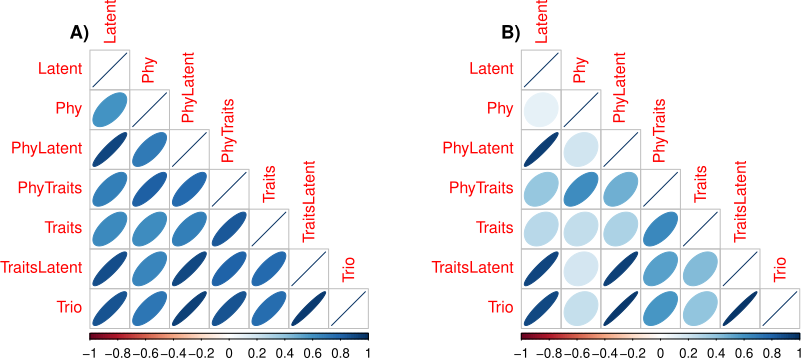
\includegraphics[width=\linewidth]{../Figs/SpearmanCorplot_nolab.pdf}
\caption{Pairwise Spearman's rank correlations of link suitabilities across models for all potential interaction (A), as well as only unobserved interactions (B). The latter set of links represents both true forbidden links, as well as other potential interactions not observed in our data-set.}
\label{fig:Figure_3}
\end{figure}









% this is a screenshot of a table, not a figure. 
%\begin{figure}%[tbhp]
%\centering
%\caption{Confusion matrix for models trained on the entire interaction network, classified assuming the average threshold value across all training interactions that maximized Youden's J statistic. Percentages represent proportions in each category out of all total links each model predicted; the absolute count of each category is represented in parenthesis. Total number of predicted links differed across models according to availability of covariant data.}
%\includegraphics[width=\linewidth]{Figs/Confusion_Matrix.pdf}
%\label{fig:Figure_4}
%\end{figure}



\end{document}
